The system performs modestly, but it is not very accurate as most scores are below 0.7, indicating a room for improvement. \\ 
\begin{table}[h!]
    \renewcommand{\arraystretch}{1.2}
   \begin{tabularx}{\columnwidth}{|>{\hsize=0.4\hsize}X| >{\hsize=0.3\hsize}X| >{\raggedright\arraybackslash\hsize=1.3\hsize}X|}
        \hline
         \textbf{Metric} & \textbf{Score} & \textbf{Insight} \\
        \hline
        BLEU & 0.503 & Exact match, may miss semantics. \\
        \hline
        ROUGE-1 & 0.639 & Measures individual term recall. \\
        \hline
        ROUGE-2 & 0.574 & Captures phrase-level matching. \\
        \hline
        ROUGE-L & 0.582 & Reflects text coherence and structure. \\
        \hline
        METEOR & 0.671 & Accounts for synonyms, better semantic capture. \\
        \hline
        BERTScore & 0.768 & Best at capturing overall semantic meaning. \\
        \hline
    \end{tabularx}
    \vspace{10pt}
    \caption{Evaluation Metrics and Their Insights}
    \label{tab:metrics}
\end{table}
\begin{itemize}
    \item BLEU (0.503) - Moderately shows word-for-word accuracy but is relatively low, indicating that the system is poor at exact matches. \\
    \item ROUGE-1 (0.639) \& ROUGE-2 (0.574) - Indicate that the system is to a certain extent capturing significant words and phrases but without good recall. \\
    \item ROUGE-L (0.582) - Means that the text generated is structurally coherent to a certain degree but is not accurate to a great extent. \\
    \item METEOR (0.671) - Better than BLEU and ROUGE since it takes synonyms into consideration, but anything less than 0.7 indicates that semantic accuracy is not high. \\
    \item BERTScore (0.768) - The highest of all, suggesting that the system is more capable of capturing semantic meaning than lexical matching, but even this score suggests that there is plenty of room for improvement. \\
\end{itemize}
\begin{figure}[h!]
    \centering
    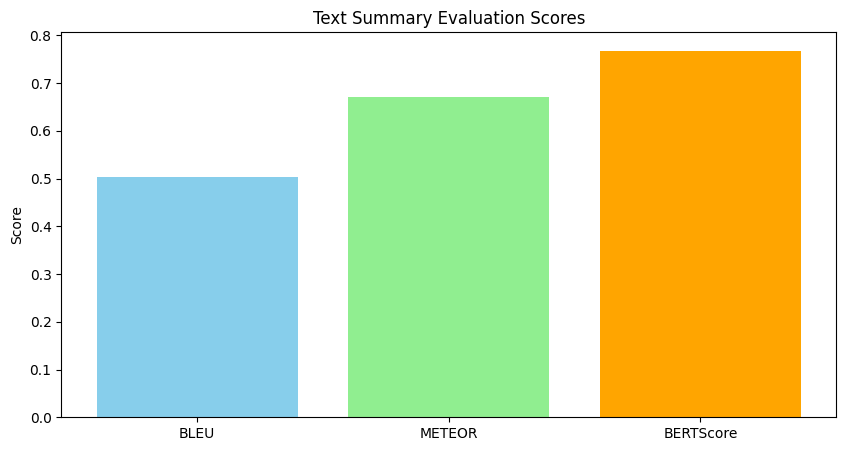
\includegraphics[width=0.5\textwidth]{fig/F1.png}
    \caption{Scores for BLEU, METEOR, and BERTScore.}
    \label{fig:f1}
\end{figure}

\begin{figure}[h!]
    \centering
    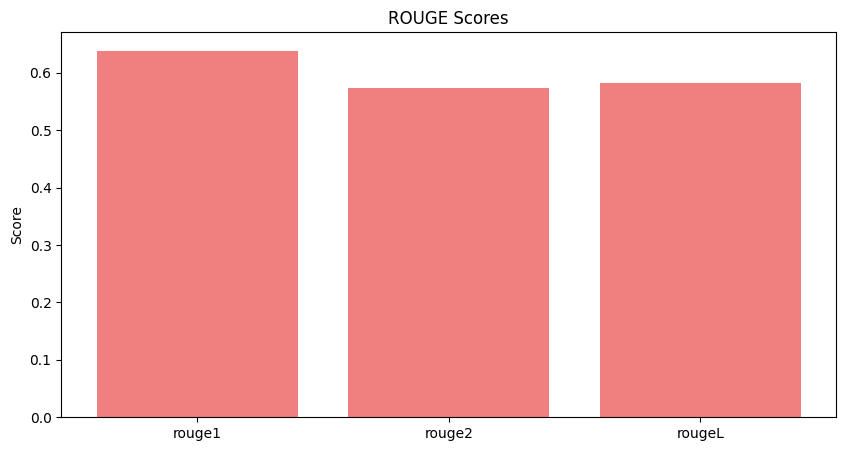
\includegraphics[width=0.5\textwidth]{fig/F2.png}
    \caption{ROUGE Scores.}
    \label{fig:f2}
\end{figure}

\begin{figure}[h!]
    \centering
    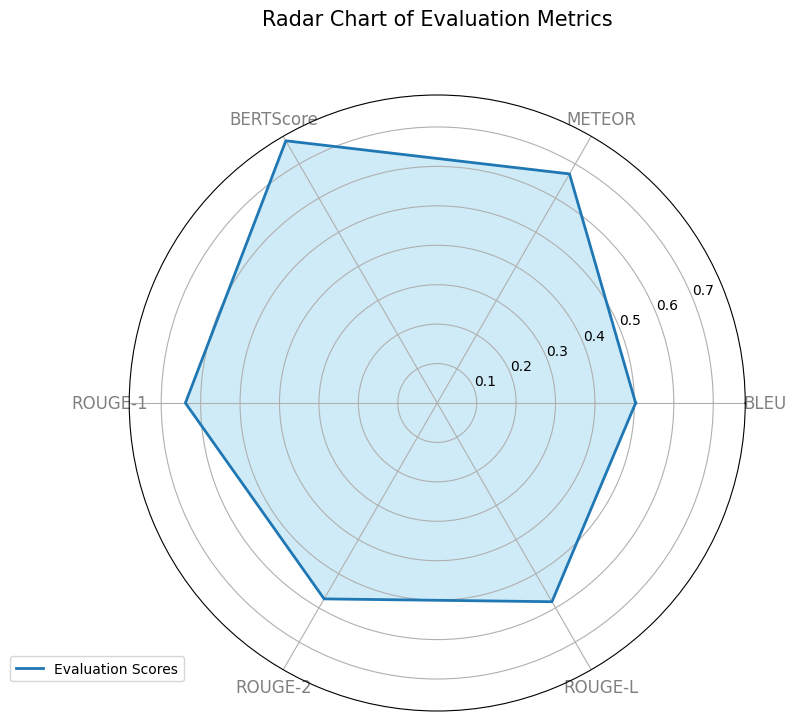
\includegraphics[width=0.5\textwidth]{fig/F3.png}
    \caption{Radar Chart of Evaluation Metrics.}
    \label{fig:f3}
\end{figure}
Comparisons \& Conclusion
Overall Performance: The system does not do very well as most scores are below 0.7, suggesting that it is not very accurate in lexical and semantic matching.
Weaknesses: BLEU and ROUGE scores are low, indicating that the generated output does not adhere to reference text closely, either in exact words or in structure.
Strengths: The system is relatively better in semantic understanding (BERTScore), but even this is not high enough to be consistently strong.
Conclusion: The system's performance is at best fair but not accurate enough. It performs badly on exact matches, recall, and structural coherence, and word choice and semantic alignment must be improved to achieve higher scores.